% Options for packages loaded elsewhere
\PassOptionsToPackage{unicode}{hyperref}
\PassOptionsToPackage{hyphens}{url}
%
\documentclass[
]{book}
\usepackage{lmodern}
\usepackage{amssymb,amsmath}
\usepackage{ifxetex,ifluatex}
\ifnum 0\ifxetex 1\fi\ifluatex 1\fi=0 % if pdftex
  \usepackage[T1]{fontenc}
  \usepackage[utf8]{inputenc}
  \usepackage{textcomp} % provide euro and other symbols
\else % if luatex or xetex
  \usepackage{unicode-math}
  \defaultfontfeatures{Scale=MatchLowercase}
  \defaultfontfeatures[\rmfamily]{Ligatures=TeX,Scale=1}
\fi
% Use upquote if available, for straight quotes in verbatim environments
\IfFileExists{upquote.sty}{\usepackage{upquote}}{}
\IfFileExists{microtype.sty}{% use microtype if available
  \usepackage[]{microtype}
  \UseMicrotypeSet[protrusion]{basicmath} % disable protrusion for tt fonts
}{}
\makeatletter
\@ifundefined{KOMAClassName}{% if non-KOMA class
  \IfFileExists{parskip.sty}{%
    \usepackage{parskip}
  }{% else
    \setlength{\parindent}{0pt}
    \setlength{\parskip}{6pt plus 2pt minus 1pt}}
}{% if KOMA class
  \KOMAoptions{parskip=half}}
\makeatother
\usepackage{xcolor}
\IfFileExists{xurl.sty}{\usepackage{xurl}}{} % add URL line breaks if available
\IfFileExists{bookmark.sty}{\usepackage{bookmark}}{\usepackage{hyperref}}
\hypersetup{
  pdftitle={How to be Careful with Covid-19 Counts: A Practical Guide to Working with Pandemic Panel Data},
  pdfauthor={Rex W. Douglass},
  hidelinks,
  pdfcreator={LaTeX via pandoc}}
\urlstyle{same} % disable monospaced font for URLs
\usepackage{longtable,booktabs}
% Correct order of tables after \paragraph or \subparagraph
\usepackage{etoolbox}
\makeatletter
\patchcmd\longtable{\par}{\if@noskipsec\mbox{}\fi\par}{}{}
\makeatother
% Allow footnotes in longtable head/foot
\IfFileExists{footnotehyper.sty}{\usepackage{footnotehyper}}{\usepackage{footnote}}
\makesavenoteenv{longtable}
\usepackage{graphicx,grffile}
\makeatletter
\def\maxwidth{\ifdim\Gin@nat@width>\linewidth\linewidth\else\Gin@nat@width\fi}
\def\maxheight{\ifdim\Gin@nat@height>\textheight\textheight\else\Gin@nat@height\fi}
\makeatother
% Scale images if necessary, so that they will not overflow the page
% margins by default, and it is still possible to overwrite the defaults
% using explicit options in \includegraphics[width, height, ...]{}
\setkeys{Gin}{width=\maxwidth,height=\maxheight,keepaspectratio}
% Set default figure placement to htbp
\makeatletter
\def\fps@figure{htbp}
\makeatother
\setlength{\emergencystretch}{3em} % prevent overfull lines
\providecommand{\tightlist}{%
  \setlength{\itemsep}{0pt}\setlength{\parskip}{0pt}}
\setcounter{secnumdepth}{5}
\usepackage{booktabs}
\usepackage{amsthm}
\makeatletter
\def\thm@space@setup{%
  \thm@preskip=8pt plus 2pt minus 4pt
  \thm@postskip=\thm@preskip
}
\makeatother
\usepackage[]{natbib}
\bibliographystyle{apalike}

\title{How to be Careful with Covid-19 Counts: A Practical Guide to Working with Pandemic Panel Data}
\author{Rex W. Douglass}
\date{2020-04-30}

\begin{document}
\maketitle

{
\setcounter{tocdepth}{1}
\tableofcontents
}
\hypertarget{intro}{%
\chapter{Executive Summary}\label{intro}}

How should we interpret the endless stream of figures and maps of COVID-19 produced by health departments and organizations around the world? For better or worse, we primarily experience large complicated events through counts- How many are dead?; How many are sick?; How many tests did we perform? These are universal questions, immediately accessible to both the producers of information like doctors and scientists and consumers of information like policy makers and citizens. For anyone who regularly works with the answers to those questions, the actual data, you know that every one of those simple numbers in a cell needs a big asterisks pointing to a long footnote explaining all of the problems in developing and using that number. This book is that footnote for COVID-19 counts. It is intended as a practical guide for using COVID-19 data, and all of the regularities and subtle gotchas you can expect to find.

This guide is built around a new resource developed at the Machine Learning for Social Science Lab called the Global Census of Covid-19 Counts (GC3). This is a single normalized and georeferenced aggregation of all of the other public aggregations of COVID-19 counts data available. We are currently aggregating 23 databases, who are in turn scraping and aggregating over ten thousand sources like public statements, news reports, and individual health department websites. Only by mosaicing all of these different resource together (782,263 observations and growing), are we able to finally provide full temporal coverage over the entire COVID-19 pandemic, and full spatial coverage over all countries in the world and in most places states/provinces as well. We are now able to track counts of confirmed cases and deaths in 4,851 locations, and number of tests performed in 1,272 locations.

This book is a deep dive into what problems and opportunities you can expect to find in these data. It is organized in order from simpler issues of data acquisition and aggregation, to more complicated questions of bias and latent true measurement.

\hypertarget{key-takeaways-tldr}{%
\section{Key Takeaways (TLDR)}\label{key-takeaways-tldr}}

You can write citations, too. For example, we are using the \textbf{bookdown} package \citep{R-bookdown} in this sample book, which was built on top of R Markdown and \textbf{knitr} \citep{xie2015}.

\hypertarget{global-covid-19-count-data}{%
\chapter{Global COVID-19 Count Data}\label{global-covid-19-count-data}}

\hypertarget{what-data-are-available}{%
\section{What data are available?}\label{what-data-are-available}}

The Global Census of Covid-19 Counts (GC3) currently aggregates 23 databases. The databases vary drastically in size, scope, collection method, and purpose. On the small end are github repositories built around collecting a single country's published statistics, often available in an unstructured form on a government website in a native language. Others are official government statistics reported directly to and compiled by international organizations, like the World Health Organization (WHO) or the European Centre for Disease Prevention and Control. Some are news organizations that collect and compile official government statistics, like the New York Times and Reuters. Nonprofits like the Covidtracking Project compile records on specific issues like testing. Wikipedia provides an interface for a massive army of volunteers to enter in statistics into tabular formats that can later be scraped. The largest and most comprehensive scraping effort is the Corona Data Scraper from the Covid Atlas which only consumes sources directly from government and health organizations (excluding news and wikipeda). These all in turn are then ingested by larger aggregation projects. Johns Hopkins University Center for Systems Science and Engineering (JHU-CSSE) is the most widely used aggregator by downstream projects. Both Microsoft's Bing research Unit and Yahoo! have in turn recently made available their knowledge graph coverage of Covid-19 counts.

Their names, links, and cleaned observation counts appear in the table below.

\hypertarget{htmlwidget-2ac2615561d17ac70794}{}

The unit of observation in our data is the location-day. The Upset plot in Figure \ref{fig:upset1} shows the number of unique location-day observations provided by each database, as well as for those available on in two datasets. Which database will provide the most unique information is difficult to tell apriori. The most unique contributions come from the Corona Data Scraper Project, which might be anticipated by their overall size. The second most unique observations however comes from Wikipedia which is surprising because our treatment of it is currently ad hoc and it should already be ingested by other sources. It goes to show that no single source, or even no small combination of sources, is sufficient to provide full temporal and spatial coverage over even this relatively brief period of the Covid-19 pandemic.

\begin{center}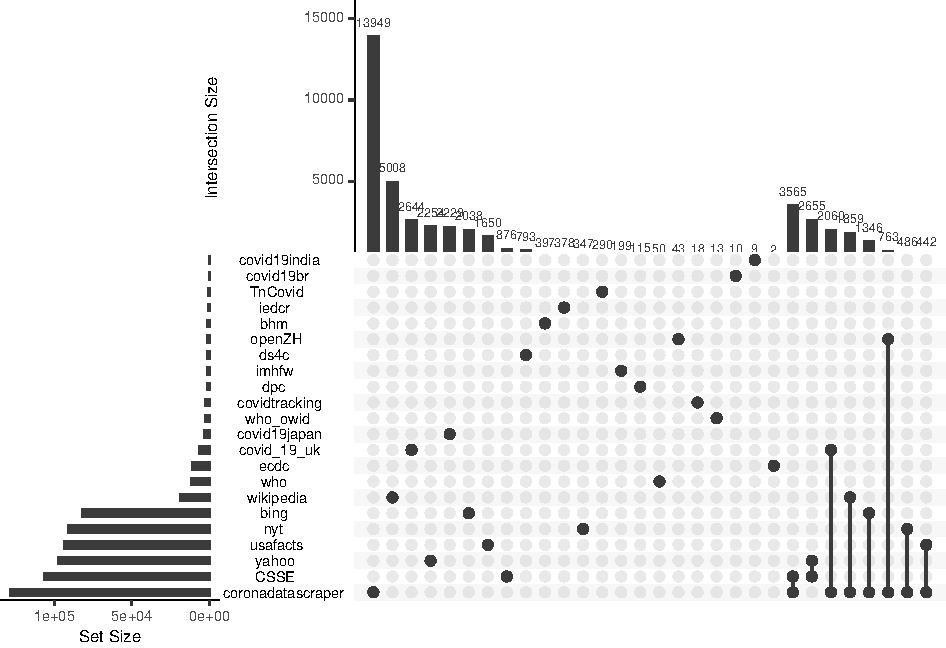
\includegraphics[width=1\linewidth]{HowToBeCarefulWithCovid19Counts_files/figure-latex/upset1-1} \end{center}

\hypertarget{what-is-their-geographic-coverage}{%
\section{What is their geographic coverage?}\label{what-is-their-geographic-coverage}}

\hypertarget{country-level-data-availability}{%
\subsection{Country Level Data Availability}\label{country-level-data-availability}}

Despite this major effort by data producers, collectors, and aggregators, there is still major geographic variation in availability across countries. Most notably in availability of counts on number of tests performed, particularly in Central Africa.

\begin{figure}

{\centering 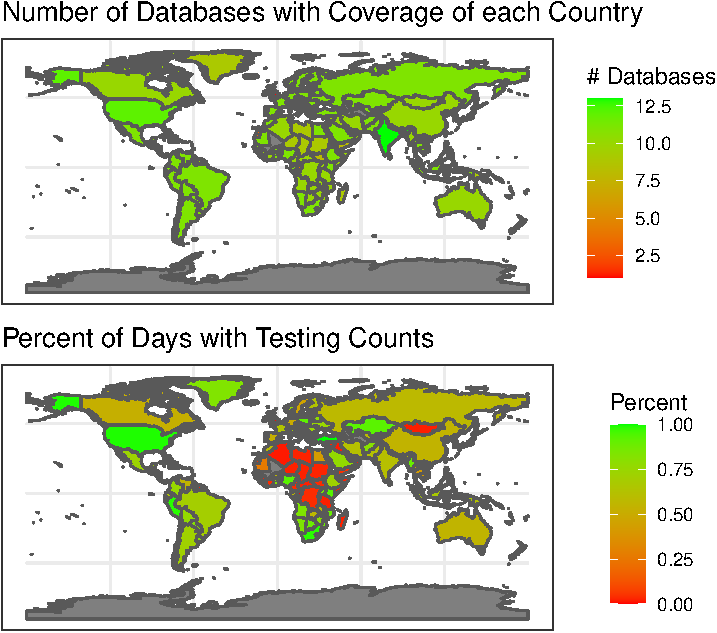
\includegraphics[width=1\linewidth]{HowToBeCarefulWithCovid19Counts_files/figure-latex/nice-fig2-1} 

}

\caption{Data coverage by country.}\label{fig:nice-fig2}
\end{figure}

\hypertarget{stateprovince-level-data-availability}{%
\subsection{State/Province Level Data Availability}\label{stateprovince-level-data-availability}}

Disparities in coverage across countries is most dramatic at the subnational level.

\begin{figure}

{\centering 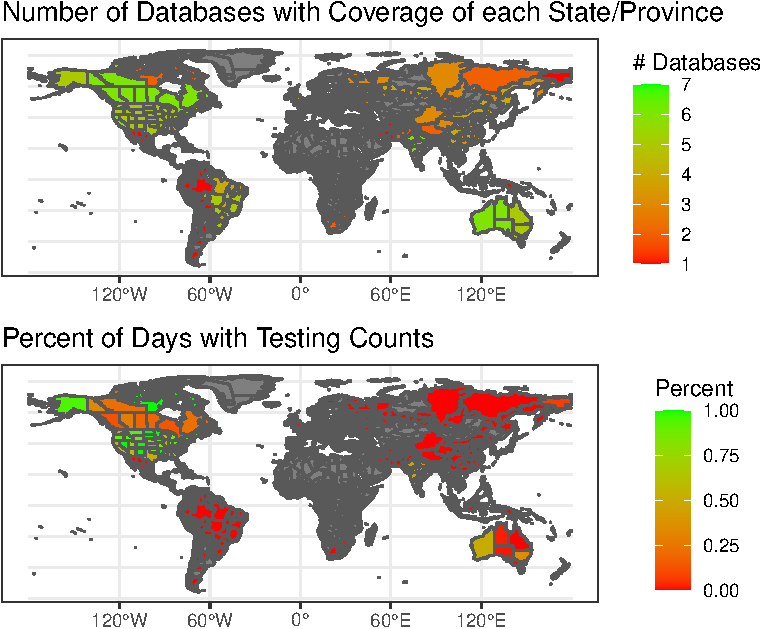
\includegraphics[width=1\linewidth]{HowToBeCarefulWithCovid19Counts_files/figure-latex/nice-fig3-1} 

}

\caption{Data coverage by State/Province}\label{fig:nice-fig3}
\end{figure}

\hypertarget{county-district-level-data-availability}{%
\subsection{County District Level Data Availability}\label{county-district-level-data-availability}}

This takes a long time to run so we're disabling it until the end

This takes a long time to run so we're disabling it until the end

\hypertarget{what-is-their-temporal-coverage}{%
\section{What is their temporal coverage?}\label{what-is-their-temporal-coverage}}

\hypertarget{comparisons}{%
\subsection{Comparisons}\label{comparisons}}

Figures x,y,z illustrate the problem of data coverage for 3 countries, China, Italy, and the U.S.

China outright refuses to release daily counts of testing. Only three databases document the beginning of the outbreak, the ECDC, the WHO, and Yahoo. On April 17, China \href{http://en.nhc.gov.cn/2020-04/17/c_79285.htm}{changed its reporting} which added 1,290 more deaths for Wuhan city only. The change is not retrospective, it shows up only a sharp discontinuity across multiple datasets.

\begin{center}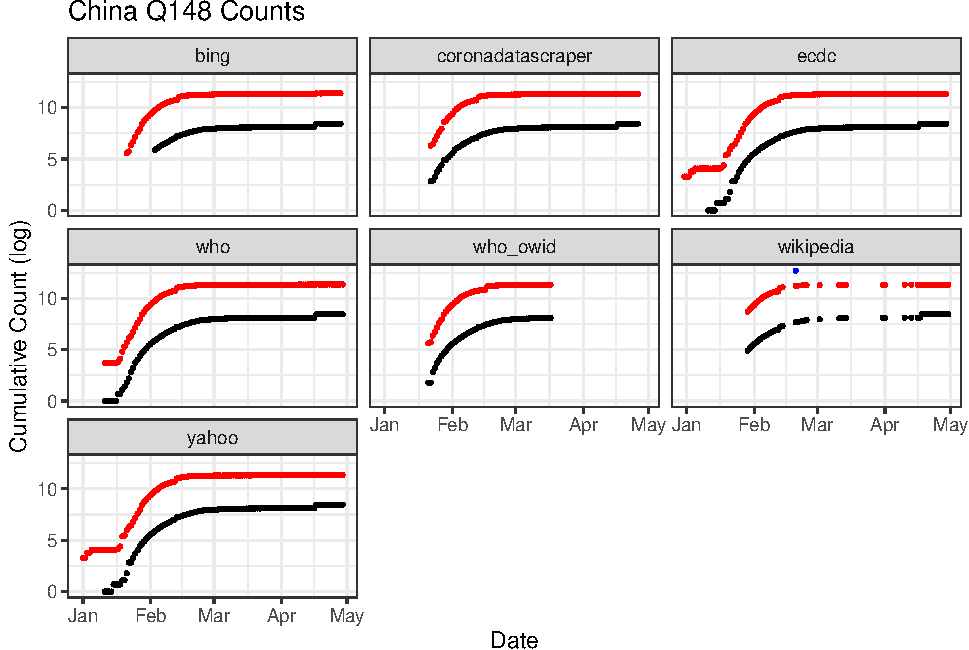
\includegraphics[width=1\linewidth]{HowToBeCarefulWithCovid19Counts_files/figure-latex/p_over_time_by_source_china1-1} \end{center}

Italy's coverage across datasets is fairly good and uniform, though there are breaks in coverage of testing for some datasets as well as variation in when each dataset starts tracking testing.

\begin{center}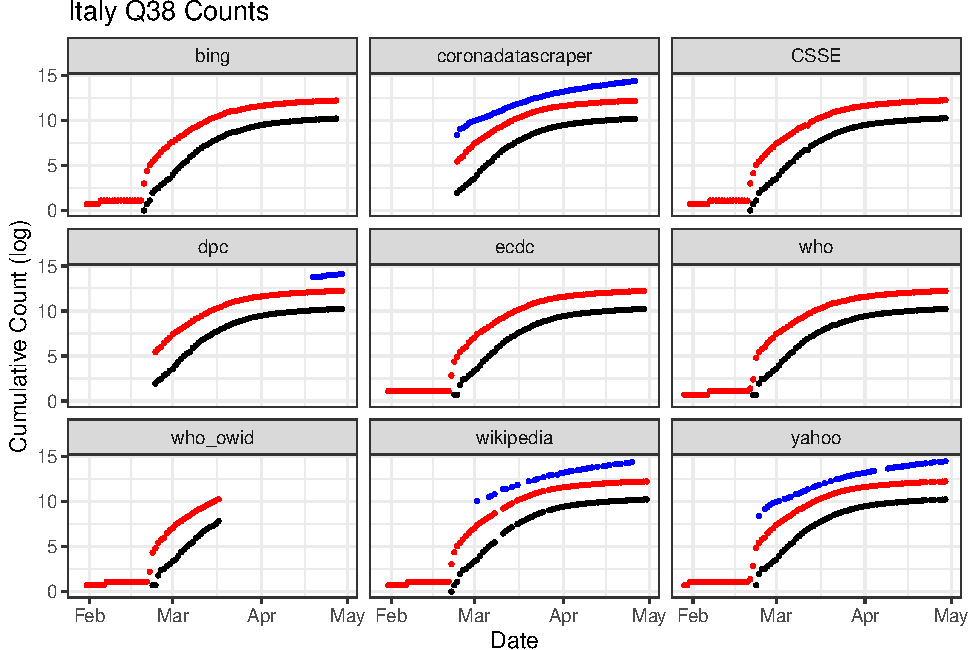
\includegraphics[width=1\linewidth]{HowToBeCarefulWithCovid19Counts_files/figure-latex/p_over_time_by_source_italy1-1} \end{center}

The U.S. has a great deal of coverage, but also a great deal of disagreement in that coverage. There is a stair step pattern in confirmed and deaths for Bing, WHO, and Wikipedia. In others reporting from day to day looks more continuous. There is also a change in reporting in late February that shows us a sharp vertical discontinuity across most datasets, though the size of the jump varies. There is also less temporal coverage of testing than is available from the caronavirus tracking project at the state level. Why those state level estiamtes aren't totaled and available at the national level is a question.

\begin{center}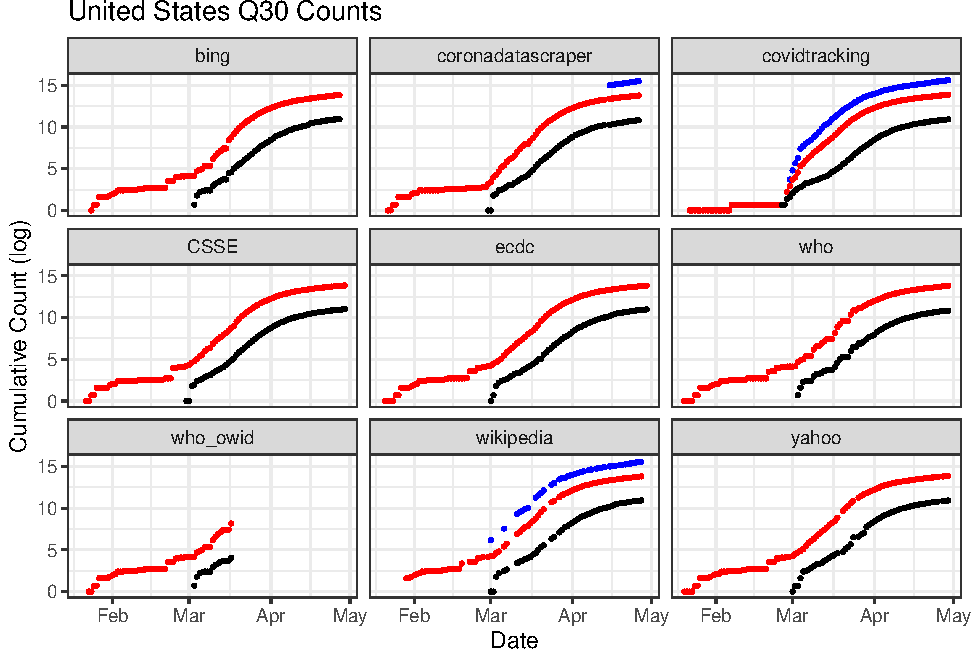
\includegraphics[width=1\linewidth]{HowToBeCarefulWithCovid19Counts_files/figure-latex/p_over_time_by_source_us1-1} \end{center}

New York has been the most heavily hit by COVID-19 in the U.S. Two sources, CornaDataScraper and the Covid Tracking Project have coverage over nearly the entire period. However, only one shows a sharp discontinuity in testing around March 10th. Digging into that disagreement more, the CTP rates New York's data release a B quality, coming from snapshots of press conferences and then switching to screenshots of New York's ``Department of Health Covid-19 Tracker'' website.

\begin{center}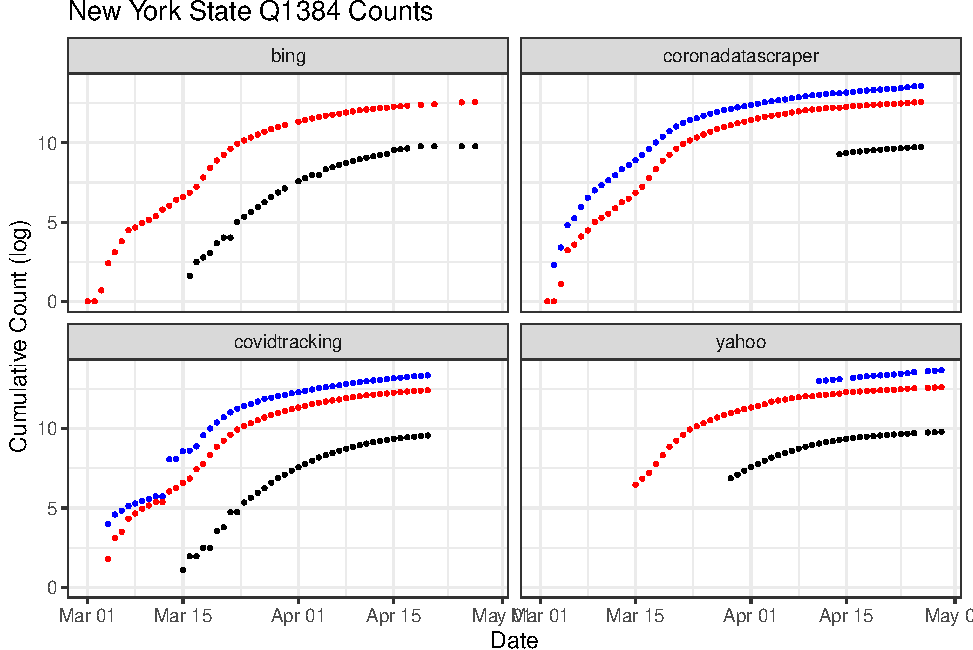
\includegraphics[width=1\linewidth]{HowToBeCarefulWithCovid19Counts_files/figure-latex/p_over_time_by_source_new_york_state1-1} \end{center}

\begin{center}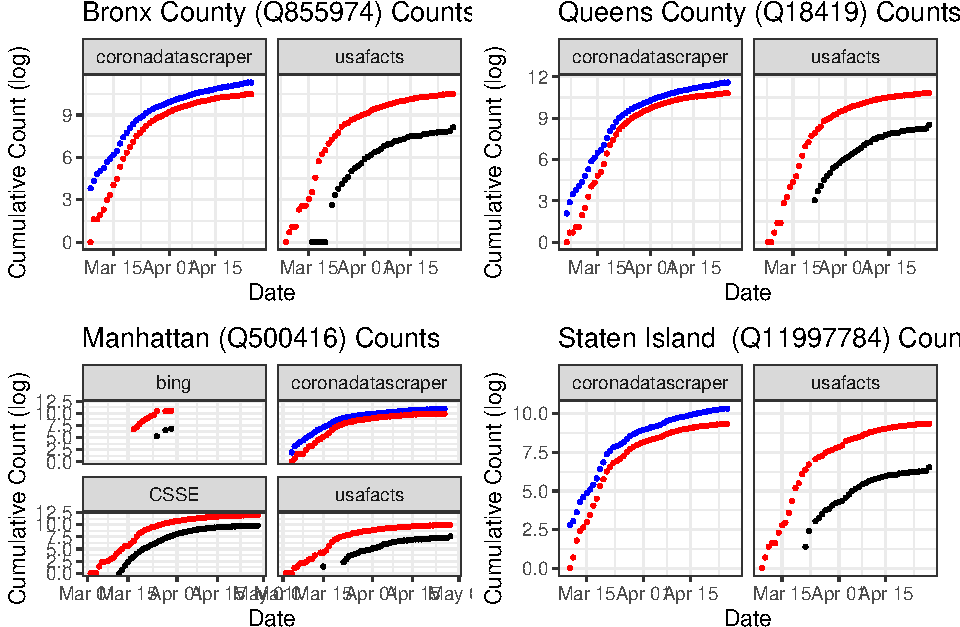
\includegraphics[width=1\linewidth]{HowToBeCarefulWithCovid19Counts_files/figure-latex/unnamed-chunk-29-1} \end{center}

\hypertarget{where-and-how-do-they-disagree}{%
\section{Where and How do they Disagree?}\label{where-and-how-do-they-disagree}}

\begin{center}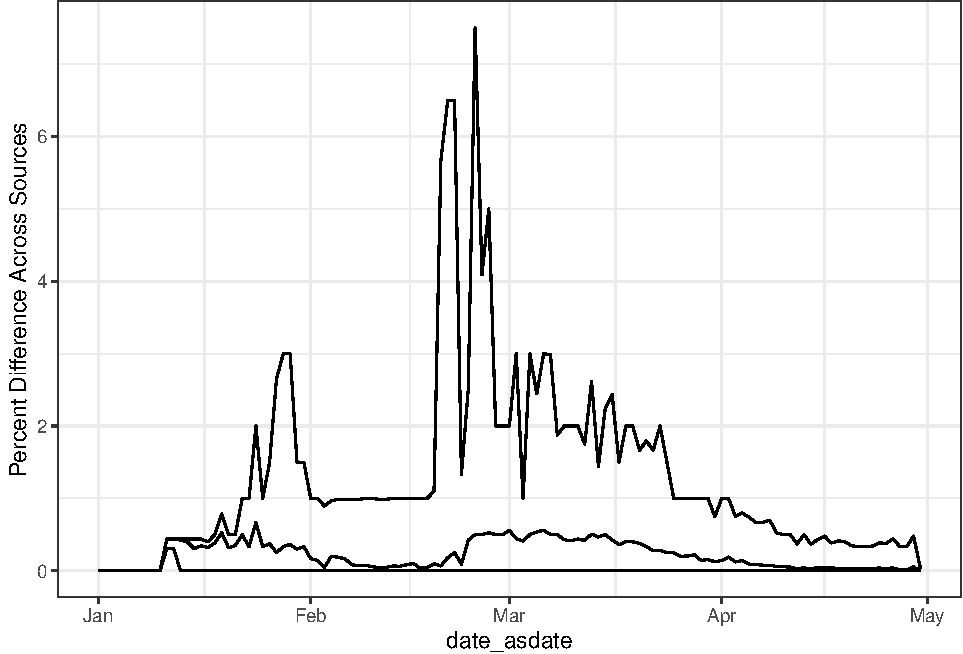
\includegraphics[width=1\linewidth]{HowToBeCarefulWithCovid19Counts_files/figure-latex/unnamed-chunk-31-1} \end{center}

\hypertarget{htmlwidget-c98470a77511f1619de2}{}

\hypertarget{htmlwidget-6bb4ad18538fc14dd23f}{}

\hypertarget{takeaways}{%
\section{Takeaways}\label{takeaways}}

Any data aggregation and cleaning approach will have to deal with the following issues

\begin{itemize}
\tightlist
\item
  Missingness

  \begin{itemize}
  \tightlist
  \item
    Prior to the first reported observation
  \item
    After the last reported observation
  \item
    Within a time series between observations
  \item
    Unbalanced across different sources
  \end{itemize}
\item
  Structural Changes

  \begin{itemize}
  \tightlist
  \item
    Changes in reporting criteria/definitions
  \item
    Changes in sourcing for unerlying data
  \end{itemize}
\item
  Disagreement

  \begin{itemize}
  \tightlist
  \item
    One or more sources report different numbers
  \end{itemize}
\item
  Errors

  \begin{itemize}
  \tightlist
  \item
    Outliers
  \item
    Merging errors
  \end{itemize}
\item
  Bias

  \begin{itemize}
  \tightlist
  \item
    Correlation between missingness and measurement
  \item
    Attenuation bias
  \end{itemize}
\end{itemize}

\hypertarget{tests}{%
\chapter{Tests}\label{tests}}

\hypertarget{tested-people-versus-tested-samples}{%
\section{Tested People versus Tested Samples}\label{tested-people-versus-tested-samples}}

\hypertarget{interpolate-within-observed}{%
\section{Interpolate Within Observed}\label{interpolate-within-observed}}

\hypertarget{interplate-prior-to-observed}{%
\section{Interplate Prior to Observed}\label{interplate-prior-to-observed}}

\hypertarget{interpolate-subnationally}{%
\section{Interpolate Subnationally}\label{interpolate-subnationally}}

\hypertarget{explaining-variation-in-testing}{%
\section{Explaining Variation in Testing}\label{explaining-variation-in-testing}}

South Korea

Vietnam
\url{https://www.reuters.com/article/us-health-coronavirus-vietnam-fight-insi-idUSKBN22B34H}

\hypertarget{common-measures-of-interest}{%
\chapter{Common Measures of Interest}\label{common-measures-of-interest}}

\hypertarget{r0-and-r}{%
\section{R0 and R}\label{r0-and-r}}

\hypertarget{case-fatality-rate-cfr}{%
\section{Case Fatality Rate (CFR)}\label{case-fatality-rate-cfr}}

\hypertarget{percent-positive}{%
\section{Percent Positive}\label{percent-positive}}

\hypertarget{deaths}{%
\chapter{Deaths}\label{deaths}}

\hypertarget{actual-infections}{%
\chapter{Actual Infections}\label{actual-infections}}

\hypertarget{conclusion}{%
\chapter{Conclusion}\label{conclusion}}

  \bibliography{book.bib,packages.bib}

\end{document}
